\documentclass[14pt]{extarticle}
\usepackage[utf8]{inputenc}
\usepackage[T1]{fontenc}
\usepackage[spanish,es-lcroman]{babel}
\usepackage{amsmath}
\usepackage{amsthm}
\usepackage{physics}
\usepackage{tikz}
\usepackage{float}
\usepackage{calc}
\usepackage[autostyle,spanish=mexican]{csquotes}
\usepackage[per-mode=symbol]{siunitx}
\usepackage{gensymb}
\usepackage{multicol}
\usepackage{enumitem}
\usepackage{setspace}
\usepackage[left=2.00cm, right=2.00cm, top=2.00cm, 
     bottom=2.00cm]{geometry}
\usepackage{Estilos/ColoresLatex}
\usepackage{makecell}
\usepackage{subcaption}
\usepackage[skip=10pt, indent=30pt]{parskip}
\usepackage{scalerel}

% \usepackage[sfdefault]{roboto}  %% Option 'sfdefault' only if the base font of the document is to be sans serif
% \usepackage[T1]{fontenc}

\usepackage{scalerel}[2016-12-29]
\def\stretchint#1{\vcenter{\hbox{\stretchto[440]{\displaystyle\int}{#1}}}}
\def\scaleint#1{\vcenter{\hbox{\scaleto[3ex]{\displaystyle\int}{#1}}}}
\def\scaleiint#1{\vcenter{\hbox{\scaleto[6ex]{\displaystyle\iint}{#1}}}}
\def\scaleiiint#1{\vcenter{\hbox{\scaleto[6ex]{\displaystyle\iiint}{#1}}}}
\def\scaleoint#1{\vcenter{\hbox{\scaleto[3ex]{\displaystyle\oint}{#1}}}}
\def\bs{\mkern-12mu}

\newcommand{\textocolor}[2]{\textbf{\textcolor{#1}{#2}}}
\sisetup{per-mode=symbol}
\decimalpoint
\sisetup{bracket-numbers = false}
\newlength{\depthofsumsign}
\setlength{\depthofsumsign}{\depthof{$\sum$}}
\newcommand{\nsum}[1][1.4]{% only for \displaystyle
    \mathop{%
        \raisebox
            {-#1\depthofsumsign+1\depthofsumsign}
            {\scalebox
                {#1}
                {$\displaystyle\sum$}%
            }
    }
}

\title{\vspace*{-2cm} Difracción  \\ Curso de Óptica \vspace{-3ex}}
\date{ }

\linespread{1.15}

\begin{document}
\maketitle

\vspace*{-2cm}

%Ref. Malacara - Óptica básica - Cap. 10 Difracción.
\section{Difracción.}

Ya se revisó que un tren de ondas no se puede acortar sin que se disperse en una multitud de frecuencias. De forma similar un frente de onda no se puede acortar en extensión transversal mediante diafragmas sin que se esparza en varias direcciones. Al primer fenómeno se le podría llamar \textit{difracción temporal} y al segundo \textit{difracción espacial}. Sin embargo, al segundo se le llama simplemente \underline{\textit{difracción}} y se ilustra en la figura (\ref{fig:figura_X_01}).
\begin{figure}[H]
    \centering
    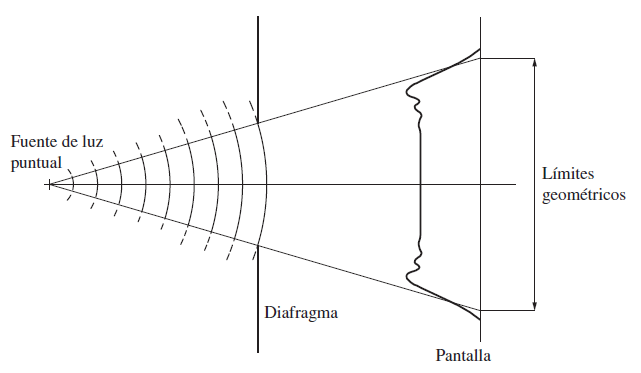
\includegraphics[scale=0.75]{Imagenes/Difraccion_01.png}
    \caption{Difracción de la luz.}
    \label{fig:figura_X_01}
\end{figure}
Como se puede ver, llega luz a la pantalla fuera de los límites de la sombra geométrica debido a este fenómeno que ahora estudiaremos. El fenómeno fue observado por primera vez en 1665 por Francesco Maria Grimaldi, quien acuñó el término difracción.

\subsection{Principio de Huygens.}

A fin de poder explicar la difracción, Christiaan Huygens propuso en los Países Bajos la regla de que \enquote{cada punto de un frente de onda se considere como una nueva fuente de ondas esféricas}. Éste es el llamado \textbf{principio de Huygens}, que se puede ilustrar por medio de la figura (\ref{fig:figura_X_02}).
\begin{figure}[H]
    \centering
    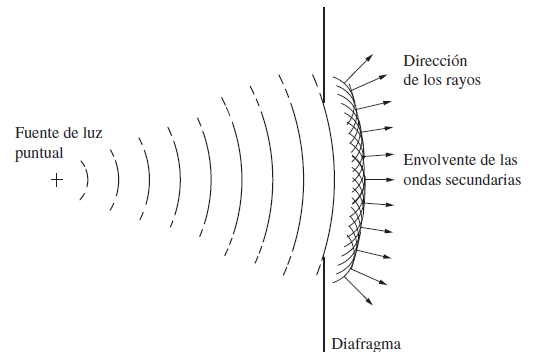
\includegraphics[scale=0.75]{Imagenes/Difraccion_02.png}
    \caption{Principio de Huygens para explicar la difracción.}
    \label{fig:figura_X_02}
\end{figure}
Según Huygens, las ondas secundarias, después de pasar por la abertura, se suman produciendo un nuevo frente de onda que casi coincide con la envolvente de dichas ondas secundarias. Esta suma de las ondas secundarias es tal que en un punto sobre su envolvente se cancelan entre sí los efectos laterales quedando sólo los que tienen la dirección de propagación de la onda. Sin embargo, esta cancelación no puede ocurrir cerca de la orilla de la obstrucción, razón por la cual la onda se esparce en varias direcciones. De esta forma se puede explicar que la luz se desvíe en las cercanías de la orilla de la abertura hacia zonas dentro de la sombra geométrica, pero no se puede sin embargo explicar el hecho de que aparezcan franjas de interferencia en las cercanías de la sombra.
\par
Augustin-Jean Fresnel modificó esta teoría más de un siglo después de que Huygens la propusiera, suponiendo que los frentes de onda secundarios no solamente se unían para formar una envolvente del frente de onda, sino que además interferirían unos con otros según los principios de la interferencia que se describieron en el capítulo anterior. Dicho de otro modo, los disturbios ópticos debidos a cada frente de onda secundario deben sumarse sobre la pantalla iluminada, tomando en cuenta su amplitud y fase en cada punto. El principio de Huygens aplicado de esta manera se conoce con el nombre de principio de Huygens-Fresnel. Esta forma de explicar la difracción tiene bastante éxito, ya que puede dar cuenta exacta de las intensidades sobre la pantalla en que se observa la difracción, incluyendo la presencia de las franjas. Sin embargo, esta teoría tiene dos defectos, uno es que no puede explicar por qué las ondas esféricas secundarias se propagan solamente en la dirección de la onda primaria y no hacia atrás. El otro es que no se obtiene con ella resultados correctos para la fase de la onda sobre la pantalla, sino desviados $\ang{90}$ con respecto a su valor real. Estas deficiencias fueron eliminadas por Kirchhoff en 1876, quien llegó esencialmente a obtener las mismas ondas secundarias que Huygens, pero en esta teoría aparecen como contribuciones diferenciales del frente de onda. No obstante, la teoría de Kirchhoff que se describirá en la siguiente sección aún es incompleta a pesar de obtener resultados sorprendentemente aproximados a la realidad. Los resultados exactos sólo se obtienen usando la teoría electromagnética.

\subsection{Teoría de la difracción de Kirchhoff.}
 
En 1876 Kirchhoff demostró que la teoría intuitiva pero muy eficaz de Huygens-Fresnel se puede justificar con un teorema integral basado en la ecuación de onda que ya estudiamos al inicio del curso. Para explicar brevemente la teoría desarrollada por Kirchhoff se comenzará por enunciar, sin demostrar, el llamado teorema de Helmholtz-Kirchhoff. La teoría comienza con el llamado teorema de Green. Consideremos una superficie cerrada arbitraria, como en la figura (\ref{fig:figura_X_03}).
\begin{figure}[H]
    \centering
    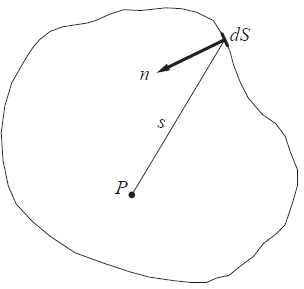
\includegraphics[scale=1]{Imagenes/Difraccion_03.PNG}
    \caption{Teorema de Helmholtz-Kirchhoff.}
    \label{fig:figura_X_03}
\end{figure}
El teorema establece que si se conoce con detalle el disturbio óptico o los valores de sus normales sobre una superficie cerrada, es posible determinar los valores del disturbio eléctrico sobre cualquier punto que se desee dentro del volumen. Este disturbio eléctrico puede ser el resultado de la iluminación producida por cualquier distribución de fuentes luminosas que pudieran estar tanto dentro como fuera del volumen encerrado por la superficie. Este teorema establece que el disturbio óptico $U (P)$ en un punto de observación $P$ cualquiera dentro del volumen está dado por:
\begin{align}
U (P) = \dfrac{1}{4 \pi} \scaleiint{6ex}_{\bs S} \left[ U \pdv{n} \left( \dfrac{e^{i k s}}{s} \right) - \dfrac{e^{i k s}}{s} \pdv{U}{n} \right] \, \dd{S}
\label{eq:ecuacion_X_01}
\end{align}
donde la integración se debe efectuar sobre toda la superficie $S$.
\par
Considerando ahora la figura (\ref{fig:figura_X_04}), supongamos que el disturbio óptico sobre la superficie es producido por una fuente luminosa monocromática puntual colocada en el punto $O$ en el exterior del volumen.
\begin{figure}[H]
    \centering
    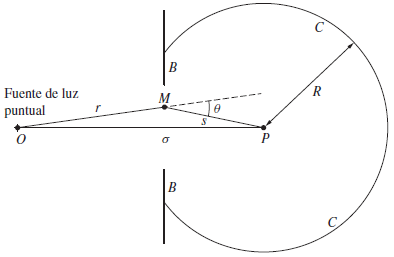
\includegraphics[scale=1]{Imagenes/Difraccion_04.png}
    \caption{Superficie para deducir la integral de Kirchhoff.}
    \label{fig:figura_X_04}
\end{figure}
Tomando en cuenta que la amplitud producida por la fuente puntual es inversamente proporcional a la distancia de dicha fuente, este disturbio sobre cualquier punto $M$ sobre la superficie cerrada quedaría dado por:
\begin{align}
U_{M} = \dfrac{A \, e^{i k r}}{r}
\label{eq:ecuacion_X_02}
\end{align}
de donde podemos encontrar que:
\begin{eqnarray}
\begin{aligned}[b]
\pdv{U_{m}}{n} &= \cos (n, r) \, \pdv{r} \left( \dfrac{A \, e^{i k r}}{r} \right) = \\[0.5em]
&=  \dfrac{A \, e^{i k r}}{r} \left( i \, k - \dfrac{1}{r} \right) \, \cos (n, r)
\end{aligned}
\label{eq:ecuacion_X_03}
\end{eqnarray}
donde $(n, r)$ es el ángulo entre la línea $r$ y la normal a la superficie. Si la distancia $r$ es mucho más grande que la longitud de onda de la luz, entonces:
\begin{align}
\dfrac{1}{r} \ll k
\label{eq:ecuacion_X_04}
\end{align}
por consiguiente:
\begin{align}
\pdv{U_{M}}{n} = \dfrac{i \, A \, k \, e^{i k r}}{r} \, \cos (n, r)
\label{eq:ecuacion_X_05}
\end{align}
y de forma análoga podemos también encontrar que:
\begin{align}
\pdv{n} \left( \dfrac{e^{i k s}}{s} \right) = \dfrac{i \, A \, k \, e^{i k s}}{s} \, \cos (n, s)
\label{eq:ecuacion_X_06}
\end{align}
Si ahora sustituimos las ecs. (\ref{eq:ecuacion_X_02}), (\ref{eq:ecuacion_X_05}) y (\ref{eq:ecuacion_X_06}) en la ec. (\ref{eq:ecuacion_X_01}), encontramos que:
\begin{align}
U (P) = \dfrac{i \, A}{2 \, \lambda} \, \scaleiint{6ex}_{\bs S} \dfrac{\exp(i \, k (r + s))}{r \, s} \, [\cos (n, s) + \cos (n, r)] \dd{S}
\label{eq:ecuacion_X_07}
\end{align}
Esta ecuación se puede ahora aplicar a la solución de problemas de difracción, tomando la superficie cerrada como se muestra en la figura (\ref{fig:figura_X_04}), donde ésta está formada por tres partes, que son el área $A$ dentro de la abertura difractora, el área $B$ sobre el diafragma, y el casquete esférico $C$ con centro en el punto de observación $P$.
\par
El disturbio $U$ sobre la región $B$ en el diafragma es cero, puesto que es opaca y la luz no pasa por ahí. Por otro lado, si el radio del casquete esférico $C$ se hace crecer hasta el infinito, la contribución de este casquete también es cero. Por lo tanto la única contribución al disturbio proviene de la abertura $\sigma$. Así, la ecuación (\ref{eq:ecuacion_X_07}) se transforma en la bien conocida integral de difracción de Kirchhoff, donde $\sigma$ es la superficie dentro de la abertura:
\begin{align}
U (P) = \dfrac{i \, A}{2 \, \lambda} \, \scaleiint{6ex}_{\bs \sigma} \dfrac{\exp(i \, k (r + s))}{r \, s} \, [\cos (n, s) + \cos (n, r)] \dd{S}
\label{eq:ecuacion_X_08}
\end{align}
Si el ángulo entre el rayo incidente y el difractado es $\theta$, como se muestra en la figura (\ref{fig:figura_X_04}), se puede ver que:
\begin{align}
\cos (n, s) + \cos (n, r) = 1 + \cos \theta
\label{eq:ecuacion_X_09}
\end{align}
y por consiguiente la integral de Kirchhoff se transforma en:
\begin{align}
U (P) = \dfrac{i \, A}{\lambda} \, \scaleiint{6ex}_{\bs \sigma} \left( \dfrac{1 + \cos \theta}{2} \right) \dfrac{\exp(i \, k (r + s))}{r \, s} \dd{S}
\label{eq:ecuacion_X_10}
\end{align}
Examinando esta expresión se pueden notar muchas similitudes pero también algunas diferencias importantes entre esta teoría y la de Huygens-Fresnel. Lo primero que podemos notar es la presencia del número complejo $i$ al frente de la integral, cuyo significado es que la fase en el punto de observación $P$ está desplazada $\ang{90}$ con respecto a la obtenida con la teoría de Huygens-Fresnel. Otra manera de decir lo mismo es que la fase de la iluminación en el punto $P$ debida a las ondas secundarias de Huygens y la fase en el mismo punto con la onda no difractada, si se quita la abertura difractora, difieren en $\ang{90}$.
\par
También es importante notar la presencia del llamado factor de inclinación $(1 + \cos \theta)/2$, el cual nos dice que la amplitud de cada onda secundaria decrece conforme aumenta el ángulo de difracción. Este factor de inclinación, que surge en forma natural en la teoría de Kirchhoff, ya había sido postulado sin bases firmes en la teoría de Huygens-Fresnel.
\par
Finalmente debe asimismo advertirse la presencia del factor $1/(rs)$, que se podría incluir también en la teoría de Huygens-Fresnel para tomar en cuenta que la amplitud decrece en forma inversamente proporcional a la distancia.
\par
Esta teoría es incompleta aún, debido principalmente a que se ignora la naturaleza transversal de las ondas luminosas. Por esta razón a esta teoría se le llama con frecuencia la \textit{teoría escalar de la difracción}. Un mayor refinamiento se ha logrado considerando la naturaleza vectorial de la luz y las propiedades electromagnéticas de los materiales difractores. Sin embargo, el problema es complicado, por lo que se han obtenido soluciones sólo en casos particulares, con geometrías relativamente simples.

\section{Difracción de Fresnel.}

Por razones históricas fundamentalmente, los fenómenos de difracción se clasifican en: a) difracción de Fresnel cuando la fuente, la pantalla o ambas se encuentran a una distancia finita de la abertura que produce la difracción, y b) difracción de Fraunhofer cuando tanto la fuente como la pantalla se encuentran a una distancia infinita de la abertura. Comenzaremos por estudiar la difracción de Fresnel para algunos casos simples pero interesantes.

\subsection{Rendija simple. Espiral de Cornu.}

Usando el principio de Huygens-Fresnel se puede encontrar el patrón de difracción de Fresnel para una rendija o abertura rectangular con ancho $S$. La geometría del problema se ilustra en la figura (\ref{fig:figura_X_05}), donde $O$ es una fuente luminosa puntual y $P$ un punto en el eje sobre la pantalla donde se desea encontrar la amplitud resultante.
\begin{figure}[H]
    \centering
    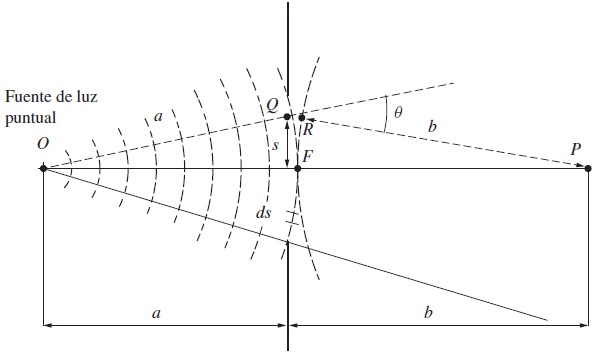
\includegraphics[scale=1]{Imagenes/Difraccion_05.png}
    \caption{Difracción de Fresnel para abertura rectangular.}
    \label{fig:figura_X_05}
\end{figure}
Se divide el frente de onda en tiras horizontales de ancho $\dd{s}$, con altura $s$, como se ilus tra en la figura (\ref{fig:figura_X_05}). La diferencia entre el camino óptico a través de $Q$ en la tira horizontal y el camino óptico a través de $F$ en el eje óptico está dada por $DCO$, y esta distancia es aproximadamente la suma de las sagitas de los arcos, del punto $Q$ al punto $R$:
\begin{align}
DCO = \dfrac{S^{2}}{2 \, a} + \dfrac{S^{2}}{2 \, b} = \dfrac{a + b}{2 \, a \, b} s^{2}
\label{eq:ecuacion_X_11}
\end{align}
Por lo tanto, la diferencia de fase entre un rayo luminoso que pasa por la abertura a una altura $s$ y el rayo axial está dada por:
\begin{align}
\delta =  k \, DCO = \dfrac{k (a + b)}{\lambda \, a \, b} s^{2}
\label{eq:ecuacion_X_12}
\end{align}

De acuerdo con el principio de Huygens-Fresnel, sumamos en forma vectorial, es decir tomando en cuenta su fase, la contribución a la amplitud de cada una de las tiras de ancho ds. La contribución de cada tira a la amplitud en el punto $P$ es directamente proporcional al ancho $\dd{s}$ de la tira. Por otro lado, si la abertura difractora es muy ancha comparada con las distancias de iluminación y de observación, debemos tomar en cuenta un factor de oblicuidad dado por:
\begin{align}
\text{Factor de oblicuidad } = \dfrac{1 + \cos \theta}{2}
\label{eq:ecuacion_X_13}
\end{align}
Este factor de oblicuidad es un postulado de Huygens, y aparece en forma natural en la teoría de Kirchhoff, como vimos en la sección anterior. Aquí se va a suponer que el ángulo $\theta$ es muy pequeño y que por lo tanto no es necesario considerar este factor.
\par
Se define ahora la variable adimensional $v$ como:
\begin{align}
v = \sqrt{\dfrac{2 (a + b)}{a \, b \, \lambda}} \, s
\label{eq:ecuacion_X_14}
\end{align}
por lo tanto la diferencia de fase con respecto al rayo axial, del rayo que pasa por la tira de ancho $\dd{s}$, queda dada por:
\begin{align}
\delta = \dfrac{\pi}{2} \, v^{2}
\label{eq:ecuacion_X_15}
\end{align}
y la contribución de una tira es directamente proporcional a su ancho $\dd{s}$ y por lo tanto también a $\dd{v}$. Al sumar las contribuciones de todas las tiras hay que tomar en cuenta su fase $\delta$. Esto se puede hacer de forma gráfi ca sumando todos los vectores de magnitud $\dd{v}$ con su fase $\delta$, de esta manera se obtiene la gráfica que se muestra en la figura (\ref{fig:figura_X_06}), donde la amplitud es directamente proporcional al vector resultante $\vb{R}$.
\begin{figure}[H]
    \centering
    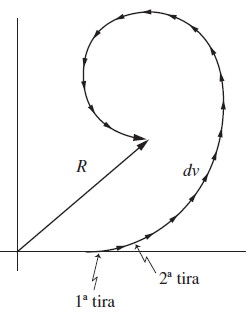
\includegraphics[scale=1]{Imagenes/Difraccion_06.png}
    \caption{Resultante vectorial de cada elemento del frente de onda en la difracción.}
    \label{fig:figura_X_06}
\end{figure}
Es posible siguiendo este método generar una curva que se pueda usar para encontrar la amplitud en el punto $P$, para cualquier ancho y posición de la rendija difractora. Utilizando la variable adimensional $v$ podemos encontrar:
\begin{eqnarray}
\dd{x} &= \dd{v} \, \cos \delta = \cos \left( \dfrac{\pi \, v^{2}}{2} \right) \dd{v} \label{eq:ecuacion_X_16} \\[0.5em]
\dd{y} &= \dd{v} \, \sin \delta = \sin \left( \dfrac{\pi \, v^{2}}{2} \right) \dd{v} \label{eq:ecuacion_X_17}
\end{eqnarray}
Por lo tanto, al integrar, la espiral de Cornu quedaría definida por:
\begin{align}
x = \scaleint{6ex}_{\bs 0}^{v} \cos \left( \dfrac{\pi \, v^{2}}{2} \right) \dd{v}
\label{eq:ecuacion_X_18}
\end{align}
y
\begin{align}
y = \scaleint{6ex}_{\bs 0}^{v} \sin \left( \dfrac{\pi \, v^{2}}{2} \right) \dd{v}
\label{eq:ecuacion_X_19}
\end{align}
Éstas son las llamadas integrales de Fresnel, cuyo valor numérico se da en tablas. La curva que se obtiene es la llamada espiral de Cornu, que se muestra en la figura (\ref{fig:figura_X_07}).
\begin{figure}[H]
    \centering
    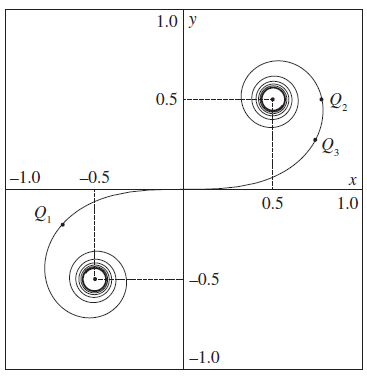
\includegraphics[scale=1]{Imagenes/Difraccion_07.png}
    \caption{Espiral de Cornu.}
    \label{fig:figura_X_07}
\end{figure}

Si la rendija difractora está centrada en el eje óptico y tiene un ancho total $S$, el primer paso es calcular el valor total de $v$. Después se colocan dos puntos simétricos $Q_{1}$ y $Q_{2}$ en la espiral de Cornu, tales que su separación medida a lo largo de la espiral sea $v$. La distancia entre estos dos puntos, medida a lo largo de una línea recta, representa la amplitud de la iluminación en el punto $P$.
\par
El patrón de difracción completo de una rendija se puede encontrar moviendo el punto de observación $P$ de arriba abajo, o lo que es lo mismo, moviendo la rendija con respecto al punto $P$ de observación. Esto se hace moviendo los puntos $Q_{1}$ y $Q_{2}$ sobre la curva, de tal forma que conserven constante su distancia $v$ medida a lo largo de la curva. La distancia entre los dos puntos representa la amplitud resultante en $P$ para esa posición de la rendija. El ángulo de la recta formada por los dos puntos móviles, con el eje $x$, representaría la fase de la onda resultante, aunque no es la correcta. La figura (\ref{fig:figura_X_08}) muestra la variación de la irradiancia en el patrón de la difracción de una rendija.
\begin{figure}[H]
    \centering
    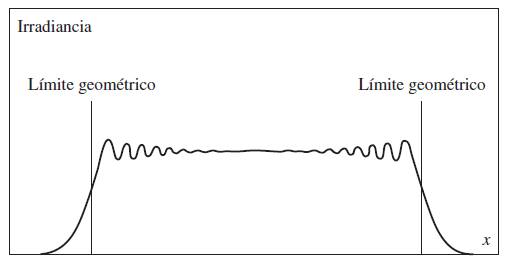
\includegraphics[scale=1]{Imagenes/Difraccion_08.png}
    \caption{Perfil de la irradiancia en la difracción producida por una rendija ancha.}
    \label{fig:figura_X_08}
\end{figure}

Para calcular el patrón de difracción de una orilla recta podemos pensar que tenemos una rendija descentrada, con una orilla sobre el eje óptico y otra al infinito. En este caso tenemos un punto fijo $Q_{3}$ y un punto móvil $Q_{2}$ en la espiral de Cornu. Así podemos obtener el patrón de difracción cuya variación en la irradiancia se muestra en la figura (\ref{fig:figura_X_09}).
\begin{figure}[H]
    \centering
    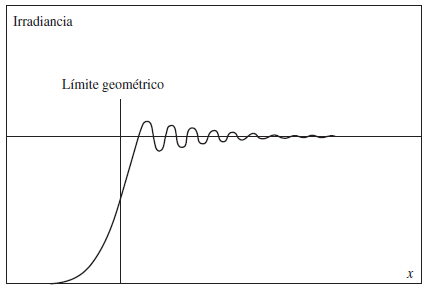
\includegraphics[scale=1]{Imagenes/Difraccion_09.png}
    \caption{Perfil de la irradiancia en la difracción producida por una orilla recta.}
    \label{fig:figura_X_09}
\end{figure}
Si la rendija se hace infinitamente ancha, es decir si no hay pantalla difractora, la amplitud en la pantalla de observación quedaría representada por la distancia entre los puntos $Q_{1}$ y $Q_{2}$. La fase de la resultante tiene entonces un valor de $\pi/4$ $(\ang{45})$ adelante de la fase que se produciría con una rendija infinitamente angosta. La razón es que según esta teoría la fase que se produce con la rendija infinitamente angosta está también $\ang{45}$ adelante de la que se produce con una pequeña perforación circular. Estas diferencias en la fase son una de las desventajas de la teoría de Huygens-Fresnel.
\par
El cálculo de patrones de difracción de Fresnel de diafragmas con contorno curvo es mucho más complicado, pero el principio físico es el mismo. La figura (\ref{fig:figura_X_10}) muestra algunos patrones de difracción de Fresnel comunes.
\begin{figure}[H]
    \centering
    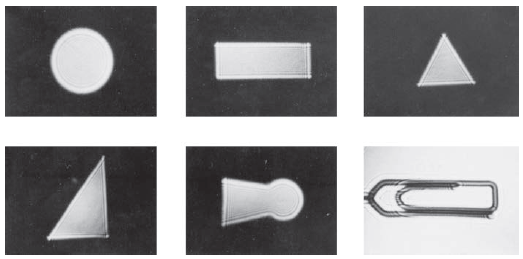
\includegraphics[scale=1]{Imagenes/Difraccion_10.png}
    \caption{Patrones de difracción de Fresnel para varios tipos de obstáculos.}
    \label{fig:figura_X_10}
\end{figure}

\subsection{Abertura circular.}

El estudio de la difracción de Fresnel de una abertura circular se puede hacer con facilidad únicamente para puntos colocados sobre el eje óptico. Al hacer esto se pueden obtener resultados muy interesantes, como veremos en seguida. Si se utiliza la misma geometría que en la figura (\ref{fig:figura_X_05}) podemos encontrar la amplitud en un punto $P$ sobre el eje de la siguiente manera. Dividimos de forma imaginaria el frente de onda en zonas concéntricas con el punto $F$, teniendo cada zona un radio promedio s distinto. Después sumamos las contribuciones de cada zona, con el fin de obtener la amplitud resultante en $P$.
\par
De la ecuación (\ref{eq:ecuacion_X_12}), la diferencia de fase entre la luz que pasa por el anillo con radio $s$ y la luz que pasa a través de su centro es:
\begin{align}
\delta = K \, s^{2}
\label{eq:ecuacion_X_20}
\end{align}
donde:
\begin{align}
K = \dfrac{\pi (a + b)}{a \, b \, \lambda}
\label{eq:ecuacion_X_21}
\end{align}
La contribución de cada zona es directamente proporcional a su área, y ésta a su vez es proporcional a su radio $s$ y a su ancho $\dd{s}$. Tomando esto en cuenta, podemos encontrar una gráfica análoga a la espiral de Cornu. Esta curva está representada por las siguientes relaciones:
\begin{eqnarray}
\dd{x} &= A \, s \, \dd{s} \, \cos \delta \label{eq:ecuacion_X_22} \\[0.5em]
\dd{y} &= A \, s \, \dd{s} \, \sin \delta \label{eq:ecuacion_X_23}
\end{eqnarray}
Ahora, diferenciando la ec. (\ref{eq:ecuacion_X_20}) podemos encontrar que:
\begin{align}
\dd{\delta} = 2 \, K \, s \, \dd{s}
\label{eq:ecuacion_X_24}
\end{align}
de donde, sustituyendo las ecs. (\ref{eq:ecuacion_X_22}) y (\ref{eq:ecuacion_X_23}), encontramos que:
\begin{align}
\dd{x} = \dfrac{A}{2 \, K} \, \cos \delta \dd{\delta}
\label{eq:ecuacion_X_25}
\end{align}
y
\begin{align}
\dd{y} = \dfrac{A}{2 \, K} \, \sin \delta \dd{\delta}
\label{eq:ecuacion_X_26}
\end{align}
de donde podemos obtener:
\begin{align}
x^{2} + \left( y - \dfrac{A}{2 \, K} \right)^{2} = \left( \dfrac{A}{2 \, K} \right)^{2}
\label{eq:ecuacion_X_29} 
\end{align}
lo cual representa un círculo con centro en el eje $y$, tangente al eje $x$ y con radio $A/2K$. Esto significa que si el radio $s$ de la abertura circular difractora se aumenta en forma continua, la amplitud en el punto $P$ oscila entre cero y un valor máximo, según se muestra en la figura ().
\begin{figure}[H]
    \centering
    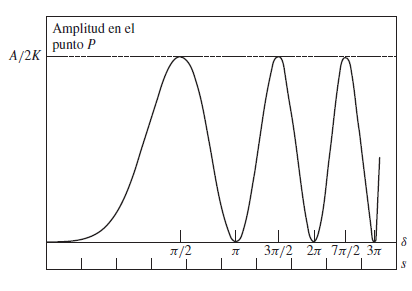
\includegraphics[scale=1]{Imagenes/Difraccion_11.png}
    \caption{Amplitud en el eje de una abertura circular.}
    \label{fig:figura_X_11}
\end{figure}
Las oscilaciones de la amplitud nunca cesan por más grande que se haga la abertura. Esto es físicamente inaceptable porque las oscilaciones deben ir amortiguándose conforme crece la abertura, hasta que se obtenga un valor al cual converja la amplitud cuando la abertura es infinitamente grande. Este problema desaparece si tomamos en cuenta el factor de inclinación $(1 + \cos \theta)/2$, ya que la amplitud $A$ y por lo tanto el radio de los círculos descritos por la ec. (\ref{eq:ecuacion_X_20}) se hacen cada vez más pequeños conforme el ángulo $\theta$ aumenta. De esta manera la curva se transforma en una espiral, como se muestra en la figura (\ref{fig:figura_X_12}).
\begin{figure}[H]
    \centering
    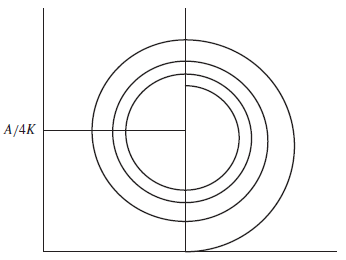
\includegraphics[scale=1]{Imagenes/Difraccion_12.png}
    \caption{Espiral de la difracción para una abertura circular.}
    \label{fig:figura_X_12}
\end{figure}
Por su parte las oscilaciones de la amplitud serían como se muestra en la figura (\ref{fig:figura_X_13}), las cuales tienden asintóticamente a un valor igual al que se obtendría sin abertura difractora o, dicho de otro modo, cuando el diámetro de su abertura es infinito.
\begin{figure}[H]
    \centering
    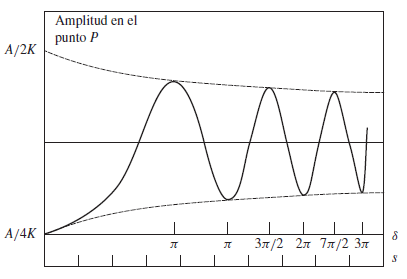
\includegraphics[scale=1]{Imagenes/Difraccion_13.png}
    \caption{Oscilación decreciente.}
    \label{fig:figura_X_13}
\end{figure}

\subsection{Placa zonal de Fresnel. Cámara de agujero.}

La amplitud para un punto en el eje de una abertura circular oscila porque algunas zonas contribuyen de manera constructiva a la interferencia, mientras que otras contribuyen de forma destructiva. Si cubrimos todas las zonas que contribuyen de forma destructiva, la amplitud es fuertemente reforzada para el punto $P$ sobre el eje que se esté considerando. A la pantalla difractora así obtenida se le llama \textit{placa zonal de Fresnel}, la cual se ilustra en la figura (\ref{fig:figura_X_14}).
\begin{figure}[H]
    \centering
    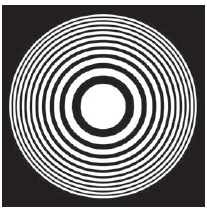
\includegraphics[scale=1]{Imagenes/Difraccion_14.png}
    \caption{Plaza zonal de Fresnel.}
    \label{fig:figura_X_14}
\end{figure}
Si la intensidad aumenta en el punto $P$, por el principio de conservación de la energía tiene que disminuir en el resto del campo. Este efecto de concentración de energía en el eje es similar al de una lente, aunque con algunas diferencias.
\par
La fase en la orilla de la zona clara central, con respecto a la del centro de la placa, es $\pi/2$, por lo tanto el radio $s$ de esta zona se puede obtener de las ecs. (\ref{eq:ecuacion_X_20}) y (\ref{eq:ecuacion_X_21}) como:
\begin{align}
s_{0} = \sqrt{\dfrac{a \, b \, \lambda}{2 (a + b)}}
\label{eq:ecuacion_X_30}
\end{align}
de donde podemos encontrar que:
\begin{align}
\dfrac{\lambda}{2 \, s_{0}^{2}} = \dfrac{1}{a} + \dfrac{1}{b}
\label{eq:ecuacion_X_31}
\end{align}
Si definimos la distancia focal $f$ de la plaza zonal de Fresnel como:
\begin{align}
f = \dfrac{2 \, s_{0}^{2}}{\lambda}
\label{eq:ecuacion_X_32}
\end{align}
podemos escribir:
\begin{align}
\dfrac{1}{f} = \dfrac{1}{a} + \dfrac{1}{b}
\label{eq:ecuacion_X_33}
\end{align}
Esta fórmula es equivalente a la fórmula de una lente delgada, que permite calcular las posiciones del objeto y de la imagen, siendo $a$ la distancia del objeto a la placa zonal y $b$ la distancia de la placa a la imagen. Solamente conviene notar aquí que la convención de signos en este caso es diferente de la usada hasta ahora para $b$.
\par
También se obtiene reforzamiento de la amplitud para otros puntos sobre el eje óptico, además del punto $P$. Por ejemplo, existe otro punto a diferente distancia del anterior, de la placa zonal de Fresnel, para el cual cada anillo claro de la placa permite pasar dos zonas anulares del frente de onda con interferencia constructiva, y una con interferencia destructiva. Por otro lado, para este mismo punto, un anillo oscuro de la placa obstaculiza dos zonas anulares con interferencia destructiva y una con interferencia constructiva.
\par
Generalizando lo anterior podemos ver que existe un reforzamiento al menos parcial de la amplitud para una multitud de puntos con orden de difracción $m$, donde cada anillo claro de la placa permite pasar $m$ zonas anulares con interferencia constructiva y $(m - 1)$ zonas anulares con interferencia destructiva. Podemos por lo tanto observar que el reforzamiento es tanto menor cuanto mayor sea $m$.
\par
En conclusión podemos decir que una placa zonal de Fresnel actúa como una lente con una multitud de distancias focales tanto positivas (convergentes) como negativas (divergentes) dadas por:
\begin{align}
f = \dfrac{2 \, s_{0}^{2}}{(2 \, m - 1) \, \lambda}
\label{eq:ecuacion_X_34}
\end{align}
donde $m$ es un entero que puede ser tanto positivo como negativo.
\par
Es posible usar una placa zonal de Fresnel o simplemente una pequeña perforación circular en lugar de una lente para formar imágenes. Por ejemplo, la llamada cámara oscura usa una pequeña perforación circular en lugar de lente para formar una imagen sobre película fotográfica. Para lograr una imagen razonablemente definida sólo es necesario que la distancia $f$ de la perforación a la imagen y el semidiámetro $s$ de esta perforación cumplan con la relación (\ref{eq:ecuacion_X_32}).

\section{Difracción de Fraunhofer. Transformadas de Fourier.}
 
Cuando la difracción se efectúa tanto con la fuente luminosa como con la pantalla de observación situadas al infinito, tenemos la llamada difracción de Fraunhofer. La fuente de luz puede estar realmente al infinito, como en el caso de una estrella, pero lo más frecuente es que esté colocada ópticamente al infinito mediante una lente colimadora. Esto se logra poniendo la fuente luminosa puntual en el foco anterior de una lente convergente, como se muestra en la figura (\ref{fig:figura_X_15}).
\begin{figure}[H]
    \centering
    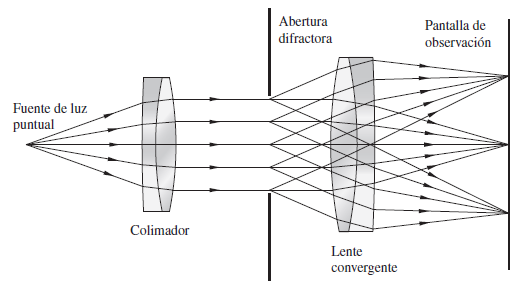
\includegraphics[scale=0.8]{Imagenes/Difraccion_15.png}
    \caption{Arreglo para producir difracción de Fraunhofer.}
    \label{fig:figura_X_15}
\end{figure}
La pantalla de observación es más difícil de colocar realmente al infinito, así que lo más frecuente es que se le coloque en el plano focal de una lente convergente como se ve en la misma figura (\ref{fig:figura_X_15}). El hecho de que la pantalla de observación esté al infi nito puede en cierto modo considerarse equivalente a decir que en la difracción de Fraunhofer lo que se observa es la distribución angular de la luz, después de la pantalla difractora.
\par
El factor de inclinación no es importante en el caso de la difracción de Fraunhofer porque los ángulos de difracción en general son pequeños. Por lo tanto, si tomamos el caso de incidencia normal ($r$ = constante), la ecuación (\ref{eq:ecuacion_X_10}) (integral de Kirchhoff) queda:
\begin{align}
U (P) = \dfrac{i}{\lambda} \, \scaleiiint{6ex}_{\bs \sigma} B \, \dfrac{e^{i k s}}{s} \dd{S}
\label{eq:ecuacion_X_35}
\end{align}
donde $B$ es una constante directamente proporcional a la amplitud sobre el plano de la pantalla difractora. Si esta pantalla difractora está colocada sobre el plano $x-y$ y la amplitud en este plano es función de $x$ y de $y$, podemos considerar que $B$ no es una constante, sino una función de $x, y$. La integral se efectúa sobre la abertura difractora. La distancia $s$ es la distancia del punto $(x, y)$ sobre la abertura al punto de observación. Esta distancia es lo suficientemente variable como para producir cambios en la fase $k s$, pues bastan variaciones del orden de una fracción de la longitud de onda para producirlas, pero lo suficientemente constante como para considerar el factor $1/s$ el mismo para todos los puntos $(x, y)$ e incluirlo como una constante multiplicadora de la función $B (x, y)$. Así, si la amplitud no es constante sobre la abertura, escribimos:
\begin{align}
U (P) = \dfrac{i}{\lambda} \, \scaleiint{6ex}_{\bs \sigma} B (x, y) \, e^{i k s} \dd{x} \dd{y}
\label{eq:ecuacion_X_36}
\end{align}
Consideremos ahora una onda difractada en una cierta dirección, como se muestra en la figura (\ref{fig:figura_X_16}).
\begin{figure}[H]
    \centering
    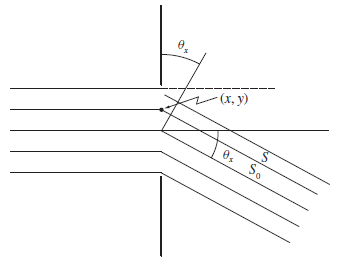
\includegraphics[scale=1]{Imagenes/Difraccion_16.png}
    \caption{Trayectorias de los rayos en la difracción de Fraunhofer.}
    \label{fig:figura_X_16}
\end{figure}
Aquí, la distancia recorrida por un rayo luminoso que sale de un punto $(x, y)$ en la abertura al punto de observación situado al infinito es $s$, y la distancia recorrida por el rayo luminoso que sale del centro de la abertura donde tomamos el origen es $s_{0}$. Así, se puede escribir la diferencia de camino óptico con respecto a la distancia recorrida por el rayo luminoso que sale de la parte central de la abertura como $DCO = s - s_{0}$.
\par 
Por lo tanto, podemos reescribir la ecuación (\ref{eq:ecuacion_X_36}) como:
\begin{align}
U (P) = \dfrac{i}{\lambda} \, \scaleiint{6ex}_{\bs \sigma} B (x, y) \, e^{i k s_{0}} \, e^{i k DCO} \dd{x} \dd{y}
\label{eq:ecuacion_X_37}
\end{align}

Si hacemos la constante $s_{0}$ igual a cero, la exponencial dentro de la integral a la derecha de la función $B (x, y)$ se hace igual a uno, obteniendo:
\begin{align}
U (P) = \dfrac{i}{\lambda} \, \scaleiint{6ex}_{\bs \sigma} B (x, y) \, e^{i k DCO} \dd{x} \dd{y}
\label{eq:ecuacion_X_38}
\end{align}
La diferencia de camino $DCO$ se puede escribir en función de los ángulos $\theta_{x}$ y $\theta_{y}$ en las direcciones $x$ e $y$ como:
\begin{align}
DCO = x \, \sin \theta_{x} + y \, \sin \theta_{y}
\label{eq:ecuacion_X_39}
\end{align}
Por, lo tanto, definiendo:
\begin{eqnarray}
k_{x} &= k \, \sin \theta_{x} \label{eq:ecuacion_X_40} \\[0.5em]
k_{y} &= k \, \sin \theta_{y} \label{eq:ecuacion_X_41}
\end{eqnarray}
podemos escribir la ecuación (\ref{eq:ecuacion_X_36}) en la forma:
\begin{align}
U (P) = \dfrac{i}{\lambda} \, \scaleiint{6ex}_{\bs \sigma} B (x, y) \, e^{i (k_{x} \, x + k_{y} \, y)} \dd{x} \dd{y}
\label{eq:ecuacion_X_42}
\end{align}
Si recordamos las transformadas de Fourier, vemos la gran similitud de esta expresión con la de una transformada de Fourier. Del teorema de Fourier, aquí, si tenemos una función $B (x, y)$ y definimos otra función $U (k_{x}, k_{y})$ como en la ecuación (\ref{eq:ecuacion_X_42}), es posible demostrar que la función $B (x, y)$ se puede escribir como:
\begin{align}
B (x, y) = \dfrac{i}{\lambda} \, \scaleto{\displaystyle\int_{-\infty}^{\infty}}{6ex} \scaleto{\displaystyle\int_{-\infty}^{\infty}}{6ex} \, U (k_{x}, k_{y}) \, e^{-i (k_{x} x + k_{y} y)} \dd{k_{x}} \dd{k_{y}}
\label{eq:ecuacion_X_43}
\end{align}
donde las funciones $B (x, y)$ y $U (k_{x}, k_{y})$ son transformadas bidimensionales de Fourier, una de la otra.
\par
Si ahora suponemos que la amplitud $B (x, y)$ está definida sobre todo el plano de la pantalla difractora y que es cero en las regiones no transparentes de ella, la región de integración se puede ampliar a todo el plano. Por lo tanto, excepto por un factor de fase constante y otras constantes multiplicativas, podemos observar que el patrón angular de difracción de Fraunhofer es la transformada de Fourier de la función de amplitud sobre la pantalla difractora. Es interesante hacer notar que esta teoría para la difracción de Fraunhofer se puede generalizar para considerar que el frente de onda sobre la abertura no es necesariamente plano, sino que puede ser ligeramente esférico o tener deformaciones. Por lo tanto, de manera general la función $B (x, y)$ podría expresarse como una función compleja de la siguiente manera:
\begin{align}
\begin{aligned}{b}
B (x, y) &= B_{0} (x, y) \, e^{- i \phi (x, y)} \\
&= B_{0} (x, y) \, e^{- i \, k \, W (x, y)}
\end{aligned}
\label{eq:ecuacion_X_44}
\end{align}
donde $B_{0} (x, y)$ es una función real que describe las variaciones de la amplitud sobre la pupila, $\phi (x, y)$ son las variaciones de la fase y $W (x, y)$ son las deformaciones del frente de onda, sobre la pupila. En los casos particulares se considera por simplicidad que $B (x, y)$ es una constante, es decir, que el frente de onda es plano y con amplitud constante.
\par
Ya hemos dicho que a fin de observar este patrón de difracción es necesaria una lente convergente que coloque ópticamente la pantalla de observación al infinito, como se muestra en la figura (\ref{fig:figura_X_17}\ref{sub@fig:figura_X_17a}).
\begin{figure}[H]
    \begin{subfigure}{0.5\linewidth}
        \centering
        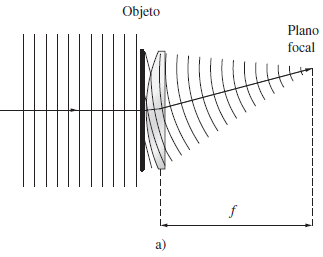
\includegraphics[scale=0.8]{Imagenes/Difraccion_17a.png}
        \caption{Arreglo con el factor de fase.}
        \label{fig:figura_X_17a}
    \end{subfigure}%
    \begin{subfigure}{0.5\linewidth}
        \centering
        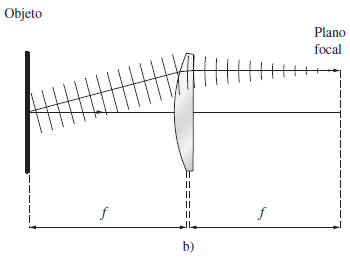
\includegraphics[scale=0.8]{Imagenes/Difraccion_17b.png}
        \caption{Arreglo sin el factor de fase.}
        \label{fig:figura_X_17b}
    \end{subfigure}
    \caption{Aparición de un factor de fase esférica en la difracción de Fraunhofer.}
    \label{fig:figura_X_17}
\end{figure}
Sin embargo, el patrón de difracción así observado tiene un factor de fase esférico, debido a que del centro de la lente a diferentes puntos del plano focal de la lente no hay una distancia constante. Este factor, sin embargo, se puede eliminar si la pantalla difractora se coloca en el plano frontal de la lente, según se muestre en la figura (\ref{fig:figura_X_17}\ref{sub@fig:figura_X_17b}). 

\subsection{Rendija simple y abertura rectangular.}

A continuación se verán algunos de los ejemplos más importantes de la difracción de Fraunhofer. Comenzaremos con los producidos por una rendija simple y por una abertura rectangular. Consideremos una rendija en el plano $x-y$, centrada en el eje $y$. Si la rendija tiene un ancho $2 \, a$, podemos escribir la ecuación (\ref{eq:ecuacion_X_42}) en la forma:
\begin{align}
U \left( k_{x} \right) = A \, \scaleint{6ex}_{\bs -\infty}^{\infty} \, e^{i k_{x} x} \dd{x}
\label{eq:ecuacion_X_45}
\end{align}
donde suponemos que la amplitud $A (x)$ permanece constante dentro de la rendija y absorbiendo la constante $i/\lambda$ dentro de la constante $A$. Así, integrando obtenemos:
\begin{align}
U \left( k_{x} \right) = A \, a \, \left( \dfrac{e^{i k_{x} a} - e^{-i k_{x} a}}{2 \, i \, k_{x} a} \right)
\label{eq:ecuacion_X_46}
\end{align}
por lo que con el empleo de la relación de Cauchy se puede obtener:
\begin{align}
U \left( k_{x} \right) = U_{0} \, \dfrac{\sin (k \, a \, \sin \theta)}{k \, a \, \sin \theta}
\label{eq:ecuacion_X_47}
\end{align}
donde $U_{0}$ es una constante. La figura (\ref{fig:figura_X_18}) muestra esta amplitud y su intensidad correspondiente como función de $k \, a \, sen \theta$.
\begin{figure}[H]
    \centering
    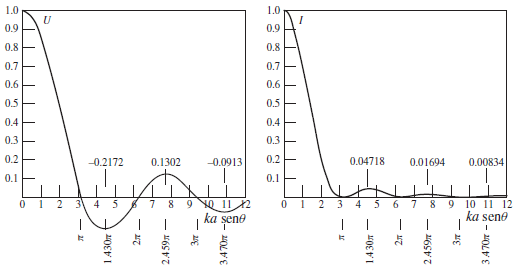
\includegraphics[scale=0.8]{Imagenes/Difraccion_18.png}
    \caption{Perfil del patrón de difracción de Fraunhofer para una rendija.}
    \label{fig:figura_X_18}
\end{figure}
Se puede ver que la primera franja oscura aparece a un ángulo $\theta$ del eje dado por:
\begin{align}
\sin \theta = \dfrac{\lambda}{2 \, a}
\label{eq:ecuacion_X_48}
\end{align}
De aquí se puede ver que el patrón de difracción se hace más angosto cuando el diámetro $2 \, a$ de la rendija crece.
\par
Por analogía con la rendija, para una abertura rectangular con ancho $2 \, a$ y longitud $2 \, b$ podemos obtener:
\begin{align}
U \left( \theta_{x}, \theta_{y} \right) = U_{0} \, \left( \dfrac{\sin (k \, a \, \sin \theta_{x})}{k \, a \, \sin \theta_{x}} \right) \left( \dfrac{\sin (k \, b \, \sin \theta_{y})}{k \, b \, \sin \theta_{y}} \right)
\label{eq:ecuacion_X_49}
\end{align}
En la figura (\ref{fig:figura_X_19}) se muestran patrones de difracción de Fraunhofer para aberturas circular, rectangular y triangular.
\begin{figure}[H]
    \centering
    \begin{subfigure}{0.24\linewidth}
        \centering
        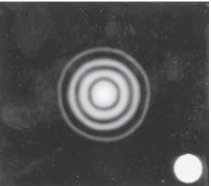
\includegraphics[scale=0.565]{Imagenes/Difraccion_19a.png}
        \caption{}
        \label{fig:figura_X_19a}
    \end{subfigure}%
    \begin{subfigure}{0.24\linewidth}
        \centering
        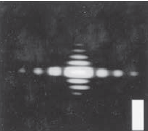
\includegraphics[scale=0.8]{Imagenes/Difraccion_19b.png}
        \caption{}
        \label{fig:figura_X_19b}
    \end{subfigure}%
    \begin{subfigure}{0.24\linewidth}
        \centering
        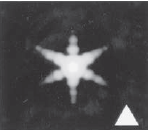
\includegraphics[scale=0.8]{Imagenes/Difraccion_19c.png}
        \caption{}
        \label{fig:figura_X_19c}
    \end{subfigure}%
    \begin{subfigure}{0.24\linewidth}
        \centering
        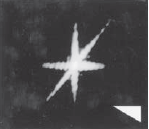
\includegraphics[scale=0.8]{Imagenes/Difraccion_19d.png}
        \caption{}
        \label{fig:figura_X_19d}
    \end{subfigure}
    \caption{Patrones de difracción de Fraunhofer: a) abertura circular, b) abertura rectangular, c) abertura triangular equilátera, y d) abertura triangular rectangular.}
    \label{fig:figura_X_19}
\end{figure}
La figura (\ref{fig:figura_X_20}) muestra la transición gradual de tres patrones de difracción de Fresnel a difracción de Fraunhofer.
\begin{figure}[H]
    \centering
    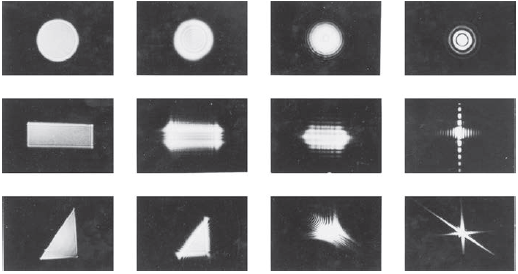
\includegraphics[scale=1]{Imagenes/Difraccion_20.png}
    \caption{Transición gradual de tres patrones de difracción de Fresnel a difracción de Fraunhofer.}
    \label{fig:figura_X_20}
\end{figure}


 


\end{document}